\section{RC Week 8}
\subsection{Data Abstraction with \texttt{class}es}
\begin{frame}{Once another look on data types: Duck typing}
Consider the problem: 
\begin{center}
	\structure{Define what a ``Duck" is?}
\end{center}
The very answer from \textit{Alex Martelli} is:
\begin{quotation}
	In other words, don't check whether it IS-a duck: check whether it QUACKS-like-a duck, WALKS-like-a duck, etc, etc, depending on exactly what subset of duck-like behaviour you need to play your language-games with.
\end{quotation}
The whole purpose of having data type is to model things. We use \texttt{struct} to model what something consists. But things are only useful when we interact with them. The \textit{observable} effects are all we care. \alert{The whole point of data abstraction is to model the behavior of objects}.
\end{frame}

\begin{frame}{Abstract Data type}
The central idea is:
\begin{center}
	\structure{Data type IS Abstraction.}
\end{center}
Always define a datatype in terms of what it can do, what kind of operations are supported for this datatype, and \alert{there should be nothing more}. Also define what you \alert{CANNOT} do with such data.
\begin{description}[Information Hiding]
	\item[Information Hiding] Actual implementation of the object is hidden away, the outside can't see, and shouldn't see what's inside.
	\item[Encapsulation] Operations become part of the type. 
	\item[Locality] Other components only depend on exposed operations (i.e. interfaces), nothing more. This is different for \texttt{struct}.
	\item[Substitutable] Change the implementable preserves program correctness.
\end{description}
\end{frame}

\begin{frame}[fragile]{Designing ADTs with \texttt{class}es}
We would like specify an Integer class:
\begin{columns}[]
	\column{.5\textwidth}

\vspace{-.2in}
\begin{minted}{c++}
class Natural {
    // OVERVIEW: An N
public:
    void  set(int v);
    // EFFECT:  ...
    // MODIFIES: this
    Natural  add(Natural v);
    Natural  mul(Natural v);
    int get();
private:
    int value;
};
Natrual num;
\end{minted}
	\column{.6\textwidth}

\vspace{-.2in}
\begin{itemize}
	\small
	\item \texttt{class} key word begins the specification of an abstract datatype. CamelCase style recommand you to capitalize first character.
	\item \texttt{public} key words begins specifying the \textit{operations}, the \textit{abstaction}, or we say the \textit{interface}. Pay attention to the \texttt{MODIFIES: this}.
	\item \texttt{private} key words calls for actual implementation.
	\item Note what's not there: a \texttt{div} method. Dividing natural numbers usually don't give you natural numbers.
	\item \texttt{num} is called an \textit{object}. \texttt{num} is an \textit{instance} of \texttt{Natural}. 
\end{itemize}
\end{columns}
\end{frame}

\begin{frame}{Implementing \texttt{class}es}
We now need to try to implement a class. We focus especially implementing class methods (member functions are usually called \textit{methods}.). 

\vspace{0.1in}
The declaration of a class is usually written in a \textit{header file}. For the example of last page we usually implement it in \texttt{natural.h}. The name of the file usually is the same as the class you are implement.  

\vspace{0.1in}
Class methods can be implemented either when you declare the class, or in a separate \texttt{.cpp} file. For our above example we usually implement it in the \texttt{natural.cpp}.

\vspace{0.1in}
Whenever you need to use a class, you include its header file. Usually each header file only contains definition of one single class, unless you have a couple of tightly related class. 
\end{frame}

\begin{frame}[fragile]{Implementing \texttt{class}es}
\begin{columns}[]
	\column{.5\textwidth}
	
	\vspace{-.3in}
	\begin{minted}{c++}
// Natural.h
#ifndef __NATURAL_H__
#defein __NATURAL_H__
class Natural {
public:
  void  set(int v) {
      this->value = v;
  }
  Natural  add(Natural v);
  Natural  mul(Natural v);
  int get() {return value;}
private:
  int value;
};
#endif __NATURAL_H__
	\end{minted}
	
	\column{.5\textwidth}
	
	\vspace{-.3in}

\begin{minted}{c++}
// Natural.cpp
#include "natural.h"
Natural 
Natural::add(Natural v) {
    Natural n; 
    n.set(value + v.get());
    return n;
}

Natural 
Natural::mul(Natural v) {
    Natural n; 
    n.set(value * v.get());
    return n;
}
\end{minted}
\end{columns}
\end{frame}



\begin{frame}[fragile]{A remark on \texttt{private}}
\texttt{private} means private to class, not to instance. 
\begin{columns}[]
\column{.42\textwidth}
	
\vspace{-.2in}
\begin{minted}{c++}
class Human {
  int leg;
public:
  int swapLeg(Human& h) {
    swap(this->leg, h.leg);
  }
  int setLeg(int n) {
    this->leg = n;
  }
};
Human h1; h1.setLeg(10);
Human h2; h2.setLeg(3);
h1.swapLeg(h2);
\end{minted}
	
	\column{.65\textwidth}
	
	\vspace{-.2in}
	\begin{itemize}
		\item Code on the left compiles and runs without problem.
		\item It's sometimes called "Since we are both human why can't I swap my leg to yours" effect.
		\item This indicates the design choice that \texttt{private} is a technique to hide abstraction implementation, other than to prevent outside modification. 
		\item Members are \alert{\texttt{private} by defualt} in a \texttt{class}. Recall that \texttt{struct} are just \texttt{class} whose member are by default \texttt{public}
	\end{itemize}
\end{columns}
\end{frame}

\begin{frame}[fragile]{\texttt{this} keyword}
\begin{columns}[]
	\column{.5\textwidth}
	
	\vspace{-.3in}
\begin{minted}{c++}
class Natural {
  int value;
public:
  int get() { 
      return value;
  }
  void set(int value) {
      this->value = value;
  }
  void printThis() {
      cout << this << endl;
  }
  // Omit other method
};
\end{minted}
	
	\column{.5\textwidth}
	
	\vspace{-.3in}
\begin{minted}{c++}
int main() {
    Natrual n1; 
    n1.printThis(); 
    cout << &n1 << endl;
    Natrual n2; 
    n2.printThis();
    cout << &n2 << endl;
}
\end{minted}

One \alert{possible} output:

\begin{minted}{text}
0x7ffff1fd2820
0x7ffff1fd2820
0x7ffff1fd2830
0x7ffff1fd2830
\end{minted}

Source under \texttt{code/rc8this}

\end{columns}
\end{frame}

\begin{frame}[fragile]{\texttt{this} keyword}
\begin{columns}[]
	\column{.45\textwidth}
	
	\vspace{-.3in}
\begin{minted}{c++}
class Natural {
  int value;
public:
  int get() { 
    return value;
  }
  void set(int value) {
    this->value = value;
  }
  void printThis() {
    cout << this << endl;
  }
  // Omit other methods
};
\end{minted}
	
	\column{.6\textwidth}
	\vspace{-.2in}
	\begin{itemize}
		\item Non-static methods always have a \texttt{this} pointer available.
		\item For non-const member methods \texttt{this} keyword is of type \texttt{ClassType*}.
		\item Members (including methods) are \alert{always} accesses through \texttt{this} keyword, either explicitly (in \texttt{set()} method), or implicitly (\texttt{get()} method).
		\item If there is an ambiguity you can use \texttt{this} to resolve ambiguity. In the \texttt{set} method, LHS refers to member and RHS refers to the argument.
	\end{itemize}
\end{columns}
\end{frame}

\begin{frame}[fragile]{\texttt{const} member function and ripple effect}
A member function can be declared as \texttt{const} to signify it will not change any member (in any possible way). The declaration must be done both in the declaration and in the implementation:

\begin{columns}
\column{.45\textwidth}

\vspace{-.25in}
\begin{minted}{c++}
// useless_class.h
class UselessClass {
    int value;
public:
    int get() const;
};
\end{minted}

\column{.55\textwidth}

\vspace{-.25in}
\begin{minted}{c++}
// useless_class.cpp
int UselessClass::get() const {
   return value;
}
\end{minted}
\end{columns}

\begin{itemize}
	\item \texttt{const} methods cannot modify any member
	\item \texttt{const} methods may only invoke other \texttt{const} methods.
\end{itemize}
You already know the basic rules of \texttt{const} methods. But unfortunately the situation (you will be facing) is much complicated (when you get to STLs). We now make a further discussion. 
\end{frame}

\begin{frame}[fragile]{\texttt{const} member function and propagation}
To illustrate the problem, we here uses a functionality called \textit{Runtime Type Info (RTTI)} to let the compiler spit out the types.

\texttt{* code/rc8const/main.cpp}
\inputminted[fontsize=\small, baselinestretch=0.865]{c++}{code/rc8const/main.cpp}	
\end{frame}

\begin{frame}{\texttt{const} member function and ripple effect}
We take down (and translate for you) the output of the program
\begin{description}[\texttt{bar()::value}]
	\item[\texttt{bar()::this}] \texttt{const} pointer to \texttt{Foo}
	\item[\texttt{bar()::value}] \texttt{const} pointer to \texttt{int}
	\item[\texttt{baz()::this}] pointer to \texttt{Foo}
	\item[\texttt{baz()::value}] pointer to \texttt{int}
\end{description}
Essentially we have the following 3 rules:
\begin{itemize}
	\item In a \texttt{const} method, \texttt{this} have type \texttt{const Class*}
	\item Non \texttt{const} member functions are not allowed to be accessed from a \texttt{const} object.
	\item Any member variable accessed through a \texttt{const}ed \texttt{this} keyword is automatically const quantified.
\end{itemize}
We provide some examples to explain them.
\end{frame}

\begin{frame}{\texttt{const} member function and ripple effect}
We take down (and translate for you) the output of the program
\begin{description}[\texttt{bar()::value}]
	\item[\texttt{bar()::this}]  pointer to \texttt{const Foo}
	\item[\texttt{bar()::value}] pointer to \texttt{const int}
	\item[\texttt{baz()::this}] pointer to \texttt{Foo}
	\item[\texttt{baz()::value}] pointer to \texttt{int}
\end{description}
Essentially we have the following 3 rules:
\begin{itemize}
	\item In a \texttt{const} method, \texttt{this} have type \texttt{const Class*}
	\item Non \texttt{const} member functions are not allowed to be accessed from a \texttt{const} object.
	\item Any member variable accessed through a \texttt{const}ed \texttt{this} keyword is automatically const quantified.
\end{itemize}
They seems very abstract. We provide some examples to explain them.
\end{frame}

\begin{frame}[fragile]{\texttt{const} ripple effect: Example }
Consider the following 2 classes
\begin{columns}

\column[]{.4\textwidth}
\vspace{-.2in}
\begin{minted}{c++}
class Integer {
  int value;
public:
  int get();
  void set(int i);
};
\end{minted}

\column[]{.6\textwidth}
\vspace{-.2in}
\begin{minted}[]{c++}
class Bar {
  Integer i;  Complicated c;
  void doComp(); // uses c
public:
  int getValue() { 
     doComp(); return i.get(); 
  } };
\end{minted}
\end{columns}

Suppose there exists a function that originally looks like:
\begin{minted}{c++}
void baz(Bar bar); // Do complicated work
\end{minted}
The function passes \texttt{Bar} by value. It was alright, until bar becomes really large. A quick fix is proposed. Somehow you know function does not modify the argument, you suggest to change it to 
\begin{minted}{c++}
void baz(const Bar& bar); // Do complicated work
\end{minted}
Pretty harmless change? What could be possibly go wrong?
\end{frame}

\begin{frame}{\texttt{const} ripple effect: Example}
Well it isn't! Let's see what happens:
\begin{itemize}
	\small
	\item We know \texttt{baz} calls \texttt{getValue} from \texttt{Bar} class. Since we change the argument to const reference. We can no long do that, since you cannot call a non-const member function on a const object.
	\item You change \texttt{Bar::getValue()} to const member function. But this gives you 2 more problems (what are they?).
	\item You tackle the easier one. Since \texttt{i} in \texttt{Bar::getValue()} is now const object, you have to change \texttt{Integer::get()} also to const member function.
	\item Another problem is \texttt{doComp()} is not const. This function does really complicated calculation with \texttt{i} and \texttt{c}. 
	\item You have no choice but to mark \texttt{Bar::doComp()} as const. This forces you inspect every member function of \texttt{Complicated} class, and change them to \texttt{const}.
	\item Now you realize this will never end! There are simply more and more things to change. You ends up rewriting the entire code base! 
\end{itemize}
\end{frame}

\begin{frame}[fragile]{\texttt{const} ripple effect: Example}
Things you observed is sometimes called the ``ripple effect" of \texttt{const} keyword: when you change $X$, you ends up changing all things related to $X$, and this goes on and \texttt{const} ends up ``infecting" everything.

There are in general 2 ways to stop this effect, both of them are dangerous and far from satisfaction.
\begin{itemize}
	\item A \texttt{const\_cast}. The programmer explicitly asks the compiler to stop checking constness and tell the compiler to trust him. 
	\item Make a non-const copy of the original object. Pass that object along. This has a obvious performance drawback.
\end{itemize}

The lesson behind this is you \alert{constness is a all-or-nothing deal}. You either do it from the begging till the end, and never at all. Constness is considered good practice. It provides very powerful assurance on correctness. So our advice is simple:
\begin{center}
	\alert{Do \texttt{const}, and do it in full scale!}
\end{center}
\end{frame}

\begin{frame}{Building source file containing classes}
We now turn to ask the question how classes are compiled. This is important for the following two reasons:
\begin{itemize}
	\item How classes are compiled are related to the memory representation of classes. Many design choices on classes are (or were) have something to do with this.
	\item You could encounter various strange problem in your project or in a real life situation. Knowing them helps to grasp the situation. 
\end{itemize}
Historically C++ was derived from a language called \textit{C With Classes}. One of the first C++ compiler will first translate C++ code into C code, then a C compiler compiles it into machine code. 

\vspace{0.03in}
We will notice that classes are (once were) merely C structures with some syntax sugar. We will also begin to notice how much trouble does the C linking strategy introduce into the language, and becomes prominent problem in its course of development. 
\end{frame}

\begin{frame}[fragile]{On compiling classes}
The code on the left will be compiled, as if, it was written in the form of the right hand side

\begin{columns}

\column{.5\textwidth}
\vspace{-.2in}
\begin{minted}[baselinestretch=.9, fontsize=\small]{c++}
class Clock {
    int hour;
public:
    void setHour(int h) {
        hour = h;
    }
    int getHour() const {
        return hour;
    }
};
void foo() {
    Clock clock; 
    clock.setHour(10);
    clock.getHour(); 
}
\end{minted}

\column{.5\textwidth}
\vspace{-.2in}
\begin{minted}[baselinestretch=.9, fontsize=\small]{c}
typedef struct Clock_t {
    int hour; 
} Clock;
void clock_setHour
       (Clock* this, int h) {
    this->hour = h;
}
int clock_getHour
       (const Clock* this) {
    return this->hour;
}
void foo() {
    Clock clock; 
    clock_setHour(&clock, 10);
    clock_getHour(&clock); 
}
\end{minted}
\end{columns}
\end{frame}

\begin{frame}{On compiling classes}
Now you should find the pattern:
\begin{itemize}
	\item Classes are arranged in memory exactly like structures. We used to say ``structures are just classes whose members are all public". On a memory point of view, it's the other way around.
	\item \alert{Methods are compiled into usual functions}, with one extra argument, the \texttt{this} keyword.
	\item Dot operator (e.g. \texttt{clock.setHour}) are translated into usual function calls.
	\item All members are accessed through the this parameter. The reason is now obvious.
	\item \texttt{const} methods results in a \texttt{const} \texttt{this}.
	\item \texttt{static} methods (if you still remember what they are), are just methods that does not take the extra argument (thus they are shared among all instances).
\end{itemize}
\end{frame}

\begin{frame}{On compiling classes: Linking}

We first go over a few things we already know about the building process (and see which of them are violated!):
\begin{itemize}
	\item Building process is mainly about compiling and linking
	\item Each source file compiles independently.
	\item Each entity must have one definition and one only (ODR).
\end{itemize}

We have looked at  look at the linking stage. 

\vspace{.05in}
Remember information about classes are ``thrown away" in the compiling stage. When it comes to linking, we are only linking function calls together. Functions are all that we care.

\vspace{.05in}	
Every class method will be turned into a function. We keep that in mind and see the following slides.
\end{frame}

\begin{frame}[fragile]{On linking classes: the setup}
\begin{columns}
\column{.45\textwidth}
	
\vspace{-.25in}
\texttt{[code/rc8class/integer.h]}
\inputminted[fontsize=\small, baselinestretch=.9]{c++}{code/rc8class/integer.h}

\texttt{[code/rc8class/integer.cpp]}
\inputminted[]{c++}{code/rc8class/integer.cpp}

\column{.55\textwidth}
	
\vspace{-.25in}
\texttt{[code/rc8class/inc.cpp]}
\inputminted[frame=single]{c++}{code/rc8class/inc.cpp}

\texttt{[code/rc8class/dec.cpp]}
\inputminted[frame=single]{c++}{code/rc8class/dec.cpp}
\end{columns}
\end{frame}

\begin{frame}[fragile]{On linking classes: the setup}
We accompany above with the following driving program

\texttt{[code/rc8class/main.cpp]}:
\inputminted[]{c++}{code/rc8class/main.cpp}

Compile the code and execute it:
\begin{minted}{text}
g++ main.cpp dec.cpp inc.cpp integer.cpp && ./a.out
\end{minted}
We observer the (not surprising) result \texttt{10 11 10}
\end{frame}

\begin{frame}{On linking classes}
We now take a step back and think. In the preprocessing stage we already knows that files included by \texttt{\#include} are copied into the file, this is (unfortunately) also true for \texttt{integer.h}:

\vspace{-0.1in}
\begin{figure}
	\centering
	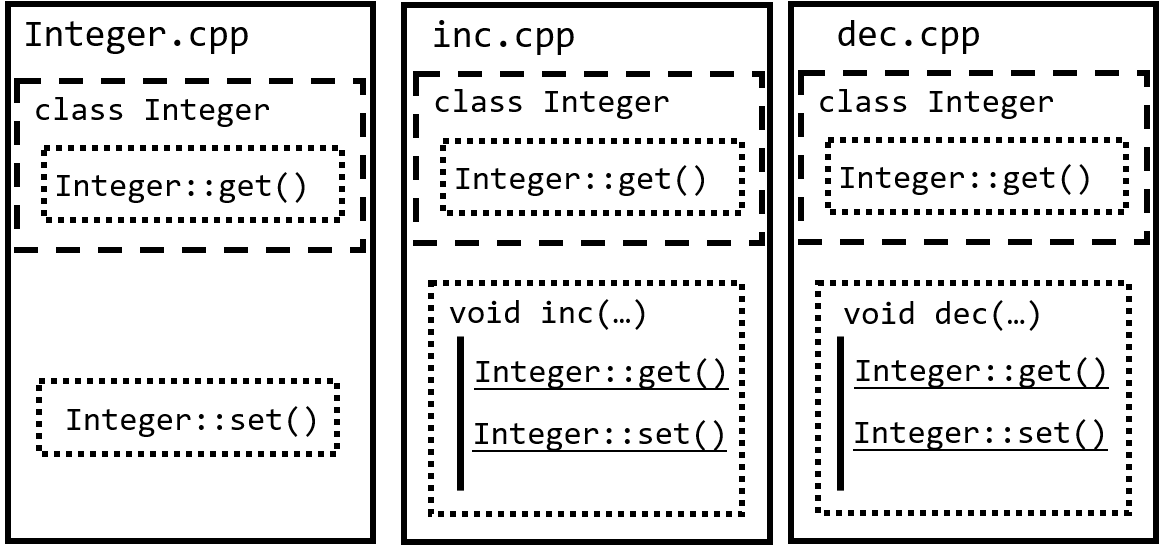
\includegraphics[scale=0.37]{fig/rc8link1}
\end{figure}

\end{frame}

\begin{frame}{On linking classes}
Pairs of the same color are linked together:
\begin{figure}
	\centering
	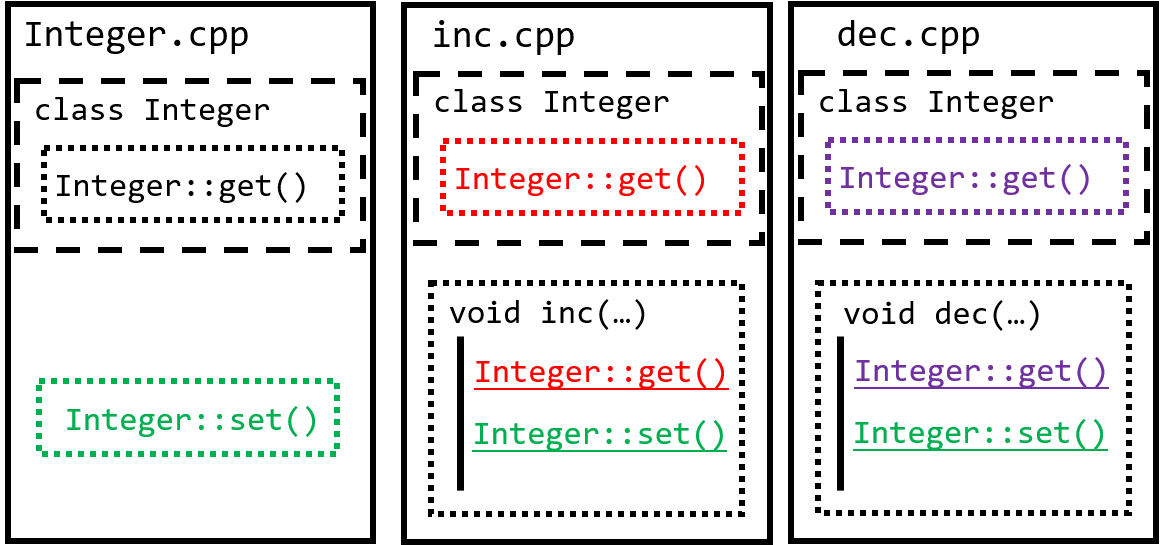
\includegraphics[scale=0.37]{fig/rc8link2}
\end{figure}
\end{frame}

\begin{frame}{On linking classes}
Thus the guideline is very simple:
\begin{itemize}
	\item Methods defined inside the class decls are linked internally.
	\item Methods defined in a separate \texttt{.cpp} source file are linked as if they are usual functions.
\end{itemize}
From a performance point of view, writing a definition of method inside the class declaration implies that the method is very simple. So instead of generating a function call whenever used the compiler will try to copy the code to each place it is used, avoiding the overhead of calling a function. This is called \textit{inlining}. 

\vspace{0.05in}
A remark we haven't made yet is \textit{abstraction always have an overhead}, a cost that we must endure to enable better flexibility. For classes, function calling mechanism is the overhead. Naturally people would want them both, i.e. ``zero cost abstraction". The way C++ achieves it is through allowing compiler to heavily optimize your code, and inlining methods is one major technique.
\end{frame}

\subsection{Working with class invariants}	
\begin{frame}{Invariants of a datatype}
We now take a look at the implementation side. From a implementation point of view, what's the difference between a list of integers, and a set of integers? 
\begin{itemize}
	\item Both of them probably are represented using an array.
	\item Both of them might need to keep track of current number of elements. 
\end{itemize} 
The major difference lies in the fact that when inserting an element, integer set must check whether the element already exists. It is the assumptions on the member that makes them different.

\vspace{0.05in}
Integer set has one more assumption than integer list. Each number in the array must be unique. Every operation of an integer set must start with this assumption, might broke it in the middle, but ends up with it.

\vspace{0.05in}
We will use your \texttt{IntSet} example in class for our discussion.
\end{frame}

\begin{frame}{Example of invariants}
\begin{columns}
	\column[]{.5\textwidth}
	
	\vspace{-.3in}
	\inputminted[fontsize=\small]{c++}{code/rc8intset/intset.h}
	
	Invariants:
	
	1) Numbers are arranged in \texttt{elts} sequentially from index zero.

	2) Number of elements in array equals to the value of \texttt{numElts}.
	
	3) Numbers are unique.
	\column[]{.6\textwidth}
	
	\vspace{-.25in}
	Guideline is:
	\begin{itemize}
		\item Methods  assume inv.s on entry.
		\item (Public) Methods must preserve inv.s on the moment of exit.
		\item Nobody cares what happens in the middle!
	\end{itemize}
	This way we safely claim invariants are always preserved for an class instance from an external point of view. 
	
	Analyze the methods:
	\begin{itemize}
		\item \texttt{insert} might broke all three.
		\item \texttt{remove} might broke 1) and 2).
		\item \texttt{const} methods will not break anything! One more advantage!
	\end{itemize}
\end{columns}
\end{frame}

\begin{frame}{Example of invariants: Implementing methods}
\begin{columns}
	\column[]{.5\textwidth}
	
	\vspace{-.3in}
	
	\inputminted[fontsize=\small,xleftmargin=1em, linenos]{c++}{code/rc8intset/intset.cpp}
	
	\column[]{.6\textwidth}
	
	\vspace{-.25in}
	
	Analyze the methods:
	\begin{itemize}
		\item L.9 checks inv.3 for uniqueness.
		\item L.7 checks inv.2 for capacity. If violation of inv cannot be recovered from, depending on how serious situation is you can \texttt{throw} or fail-fast.
		\item L.9 uses inv.1. We insert at the end, temporarily breaks invariance.
		\item L.9 operator \texttt{++} restores inv.
		\item Inv.3 ensures \texttt{remove} works.
		\item L.15 restores inv.1. L.16 restores inv.2. A significant amount of code is dedicated to preserving invs.
	\end{itemize}
\end{columns}
\end{frame}


\begin{frame}{Remarks on invariants}
We would like to note the following things:
\begin{center}
	\structure{The centric problem in choosing an implementation\\ for an ADT, is choosing the invariants.}
\end{center}
There are multiple ways to write an implementation an \texttt{IntSet} of course. The major difference of them, is they need to keep different invariants, and thus have different performance. 

For example, you have already seen \texttt{IntSet} implemented using a sorted array. The one extra invariant you need to keep is that elements are sorted. Based on that extra invariant:
\begin{itemize}
	\item Queries are much quicker.
	\item Deletion and insertion are slower (by a constant factor).
\end{itemize}
In VE281 you will see (many) other ways of implementing this IntSet, for example using hash tables, or balance trees. It is always helpful to understand what the invariant for an implementation.
\end{frame}

\begin{frame}{Invariants and bad practices}
Thinking about invariants immediately gives us hints on what are seemingly good, some even sounds terrific, but are actually pretty bad ideas. We now take a look at some of them.

\begin{description}[Alice]
	\small
	\item[Alice] I'd like to add a public method to \texttt{IntSet}, let's say \texttt{find()}, which takes an element, found it in the set, and returns an reference to that element. 
	\item [Bob] Why do you want to do that?
	\item [Alice] Well my code needs to modify elements in the array, a lot. This would significantly accelerate the process.
	\item [Bob] ...
	\item [Alice] Oh, I get it, it's a pretty bad idea. OK I have another idea, I want to add a method, \texttt{data()}, which returns the pointer to array, since my code needs to iterate through the set. 
	\item [Bob] ...
	\item [Alice] What if I return pointer to const?
	\item [Bob] ...
	\item [Alice] Well, I give up. It's not as easy as I thought.
\end{description}
\end{frame}

\begin{frame}{Invariants and bad practices}
Well Alice does have her point. Her requirements are very real and the solutions does solutions could work, but remember the words from \textit{Donald Knuth}:
\begin{quotation}
	\structure{Premature optimization is the root of all evil}.
\end{quotation}
Never trade correctness for performance in designing phase. 
\begin{itemize}
	\small
	\item 1st and 2nd change Alice proposed have the problem that the client could change the content of the internal array, without notifying the instance. There is by no means the instance can guarantee the new value won't violate uniqueness invariance.
	\item Now Alice proposes the third one. The \texttt{const} key word could prevent the element from being modified. But it exposes the implementation to outside. Now the fact that elements are stored in a linear array becomes part of the abstraction, you can no longer change that. The problem is, iterating through a set seems to be an important feature, we DO need that. Well, the correct solution is using iterators, you will know them later in this course.
\end{itemize} 
\end{frame}

\begin{frame}{Invariants and bad practices}
Well Alice does have her point. Her requirements are very real and the solutions does solutions could work, but remember the words from \textit{Donald Knuth}:
\begin{quotation}
	\structure{Premature optimization is the root of all evil}.
\end{quotation}
Never trade correctness for performance in designing phase. 
\begin{itemize}
	\small
	\item 1st and 2nd change Alice proposed have the problem that the client could change the content of the internal array, without notifying the instance. There is by no means the instance can guarantee the new value won't violate uniqueness invariance.
	\item Now Alice proposes the third one. The \texttt{const} key word could prevent the element from being modified. But it exposes the implementation to outside. Now the fact that elements are stored in a linear array becomes part of the abstraction, you can no longer change that. The problem is, iterating through a set seems to be an important feature, we DO need that. Well, the correct solution is using iterators, you will know them later in this course.
\end{itemize} 
\end{frame}

\begin{frame}{Invariants and the constructor}
\alert{Invariants are there as long as the object is there.} The earliest moment the object is created, is when it is defined. Classes, are just structures, in terms of memory. Structures contains undefined values when created, so naturally does the classes. 

\vspace{0.03in}
Think about \texttt{IntSet}, when the object is created, chances are \texttt{numElts} contains non-zero value, while your set should be empty.

\vspace{0.03in}
We need a mechanism, a function, that is invoked whenever the an instance is created. This function is called, and called always, to initialize the object, or more strictly, to setup the invariance.

\vspace{0.03in}
Such special functions are \alert{constructors}, or \alert{ctors} for short. From this point on it's important to think the initialization, not as assigning special values to member variables, but as invoking the constructor to setup invariants (together with the initial state, e.g. initialize the \texttt{IntSet} with one default element in it for whatever reason).
\end{frame}

\begin{frame}[fragile]{Constructors: Syntax}

\begin{columns}
	\column[]{.5\textwidth}
	
	\vspace{-.3in}
	The construct for \texttt{IntSet}:
	\inputminted[]{c++}{code/rc8intset/intset_ctor.h}
	
	
	\column[]{.6\textwidth}
	
	\vspace{-.65in}
	
	\begin{itemize}
		\small
		\item Ctors have same name as class.
		\item Ctors don't return anything. 
		\item Usually \texttt{public}, but could be \texttt{private} for special need.
		\item A class could have more than one ctor, depending on what the initial state should be. We say the constructor is overloaded.
		\item Ctors could take initialization list.
		\item Ctor is the first function being called when the object is created. Unfortunately ``created" is not as simple as it sounds.
		\item A ctor that does not take argument is called \texttt{a default ctor}. Every class must always have a ctor. If you don't specify \alert{any ctor}, a ctor is synthesized for you (under some conditions).
	\end{itemize}
\end{columns}
\tiny{* We left out copy/move constructors on purpose. You will learn them later.}
\end{frame}

\begin{frame}[fragile]{Constructors: Explanations}
We need to break down the words from previous slide. We first look at the first four lines. The first three seems direct. For the fourth one:
\begin{minted}{c++}
IntSet set1; // set1 is init to an empty set;
IntSet set2(10); // set2 contains single elem 10
\end{minted}

\begin{minted}{c++}
int foo(const IntSet& s1, const IntSet& s2);
foo(IntSet(), IntSet(10)); // Anymous construction
\end{minted}

Further more, latest C++ standard guarantees the following:
\begin{minted}{c++}
IntSet setx = IntSet();    // Same as set1 
IntSet sety = IntSet(10);  // Same as set2
IntSet setz = 10;          // Same as set2
\end{minted}
This is non-trivial, for reasons you will see one or two weeks later. This is called \textit{guaranteed copy elision}. Now some food for thought: 

Why \texttt{set1} is not initialized as \texttt{IntSet set1();} for consistency?
\end{frame}

\begin{frame}[fragile]{Constructors: Explanations}
We now question: Is constructor really the first function being called when created? Well that depends on how you understand ``created"! One should argue the ctor IS part of object creation.

\vspace{0.1in}
In fact, there are 4 steps (roughly) in creating an class instance.
\begin{enumerate}
	\item Allocation of space, we (in general) don't have control over.
	\item Construction of the base class object.
	\item Construction of the members of current class.
	\item Calling the constructor.
\end{enumerate}
These 4 steps goes recursively. In fact the constructor is the last function being called. This is natural. 

When the constructor is called, we should be able to use all member variables and base class. So their invariants must have been setup in advance! This is the only way things makes sense.
\end{frame}

\begin{frame}[fragile]{Initializer list: Setup}
The \textit{initializer list}, the things after colon controls the second and third step. 

\begin{minted}{c++}
ClsName::ClsName() : base(..), m1(..), m2(..) {
    // Code for the constructor goes here
}
\end{minted}

%You might wonder, wait a minute, I have never write initializer list before, I don't even write a constructor!

To better illustrate our ideas, we make some changes to our original \texttt{IntSet}, specifically 2 changes:

\begin{itemize}
	\item We add a line of output to the ctors to indicate with constructor is being called.
	\item We make 2 more ``version" of our original \texttt{IntSet}, one \texttt{OddIntSet} and \texttt{EvenIntSet}. They only allow odd and even numbers, respectively.
\end{itemize}

We now propose a slightly faster \texttt{IntSet}. This \texttt{IntSet} is composed of an \texttt{OddIntSet} and \texttt{EvenIntSet}. It dispatches the operation on integers to those two sub-\texttt{IntSet}. 
%
%Well, if you don't provide any initializer list, the compiler calls the default constructor on every ctor, if a default ctor is available. If the default ctor is not available, a compile error is thrown.
\end{frame}

\begin{frame}[fragile]{Initializer list: Setup}
The \textit{initializer list}, the things after colon controls the second and third step. 

\begin{minted}{c++}
ClsName::ClsName() : base(..), m1(..), m2(..) {
    // Code for the constructor goes here
}
\end{minted}



To better illustrate our ideas, we make some changes to our original \texttt{IntSet}, specifically 2 changes:

\begin{itemize}
	\item We add a line of output to the ctors to indicate with constructor is being called.
	\item We make 2 more ``version" of our original \texttt{IntSet}, one \texttt{OddIntSet} and \texttt{EvenIntSet}. They only allow odd and even numbers, respectively.
\end{itemize}

We now propose a slightly faster \texttt{IntSet}. This \texttt{IntSet} is composed of an \texttt{OddIntSet} and \texttt{EvenIntSet}. It dispatches the operation on integers to those two sub-\texttt{IntSet}. 
%

\end{frame}

\begin{frame}[fragile]{Initializer list: Setup II}
\begin{columns}
	\column[]{.5\textwidth}
	
	\vspace{-.3in}
	Decl. of \texttt{OddIntSet}
	\inputminted[fontsize=\small]{c++}{code/rc8init/oddintset.h}
	
	\column[]{.5\textwidth}
	
	\vspace{-.3in}
	Partial implementation:
	\inputminted[fontsize=\small]{c++}{code/rc8init/oddintset.cpp}
\end{columns}

We omit the very similar version for \texttt{EvenIntSet}.
\end{frame}

\begin{frame}[fragile]{Initializer list: Setup III}
\begin{columns}
	\column[]{.5\textwidth}
	
	\vspace{-.2in}
	Declaration of \texttt{OddIntSet}
	\inputminted[fontsize=\small]{c++}{code/rc8init/fastintset.h}
	
	\column[]{.5\textwidth}
	
	\vspace{-.2in}
	Partial implementation:
	\inputminted[fontsize=\small]{c++}{code/rc8init/fastintset.cpp}
\end{columns}

\end{frame}

\begin{frame}[fragile]{Initializer list: Example}
We create a main function and instantiate an instance of \texttt{FastIntSet}. We observe the following ouput:
\begin{minted}{text}
OddIntSet dft ctor
EvenIntSet elt ctor
fIntSet ctor
\end{minted}
This implies an initialization order of \texttt{oddSet-evenSet-ctor}. This follows from our expectation. 

\vspace{0.1in}
A (not so important) remark we would like to make is
\begin{itemize}
	\item The order of initialization of the members is guaranteed by standard. It's NOT a UB!
	\item Contrary to intuition \textit{it is not specified by initializer list}, but by the order they appear in the declaration.
	\item Base objects are guaranteed to be initialized before members.
	\item We recommend you to specify the init-list in the same order as the declaration, for clearance.
\end{itemize}
\end{frame}

\begin{frame}[fragile]{Initializer list: Default initialization}
We now make a tiny change to the original setup. We change the ctor for \texttt{FastIntSet} to 
\begin{minted}{c++}
FastIntSet::FastIntSet() 
    : oddSet() {cout << "fIntSet ctor\n";}
\end{minted}

Oops, we forgot to specify initializer for \texttt{evenSet}.

\begin{minted}{text}
OddIntSet dft ctor
EvenIntSet dft ctor
fIntSet ctor
\end{minted}

\texttt{evenSet} is still initialized, no surprise, otherwise the invariant for \texttt{oddSet} would be broken. Members are default constructed, if they don't appear in the initializer list. We could even simply write 

\begin{minted}{c++}
FastIntSet::FastIntSet() {cout << "fIntSet ctor\n";}
\end{minted}

Which will produce the same result. Now what about members like \texttt{int}? Well, you can think of them as a class, whose default constructor does nothing at all!
\end{frame}

\begin{frame}[fragile]{Initializer list: Default initialization}
We can even leave out the constructor for \texttt{FastIntSet} entirely. In which case we would have the following output.

\begin{minted}{text}
OddIntSet dft ctor
EvenIntSet dft ctor
\end{minted}

Essentially the compiler would synthesize (create) and constructor for you, whose initializer list initializes everything using their default constructor.  

You might wonder, wait a minute, I have never write initializer list before, I don't even write a constructor before this lesson! That's how you ``get away" with writing constructors before!

Modern design principal is against leaving things unspoken. If you believe you only need a default constructor, you could do:

\begin{minted}{c++}
IntSet::InSet() = default; // In class decl.
\end{minted}

Next up we will look at something that is not taught in class, but problems you will meet in your own struggle with C++.
\end{frame}

\begin{frame}[fragile]{Initializer list: Default initialization}
We first change the ctor of \texttt{FastIntSet} to 
\begin{minted}{c++}
FastIntSet::FastIntSet() 
    : oddSet() {cout << "fIntSet ctor\n";}
\end{minted}

Then we \textbf{remove the default ctor} for \texttt{EvenIntSet}.

We compile the program. The question is what SHOULD happen?

\pause
\vspace{0.1in}
From a design point of view, if a class does not provide a default constructor, indicates the class is not (more likely should not be) default constructible, there is no way to setup a invariance without supplying an argument. Think about it, what should be the default skin color for an instance of a human class? None.

In this case, any reasonable design would require an compile error is thrown. This is exactly the case. They compiler will look for \texttt{evenIntSet::evenIntSet()} and reports a not-found error. \alert{Situation is similar if you leave out the entire ctor of \texttt{FastIntSet}.}
\end{frame}

\begin{frame}{Why initializing in initialization list is better?}
You are asked this question in the lecture slides but the question is left unanswered in the lecture slides.

\vspace{0.1in}
Frankly the questions really should be the other way around: on what grounds do initialization in the code is better? I can think of the following reasons you should prefer (in some cases you have to use) initialization list:
\begin{itemize}
	\item Performance. This will be discussed later on. In some cases the performance could be significant.
	\item Exception safety. We will discuss this when we you learn the rule of big three (five, actually).
	\item A member that don't have a default constructor must be initialized in the initialization list.
	\item \texttt{const} members and references can only be initialized in the initialization list.
	\item Semantic reasons.
\end{itemize} 
\end{frame}

\begin{frame}[fragile]{Comments on the performance argument}
A final comment on the performance argument. Suppose we write 
\begin{minted}{c++}
FastIntSet::FastIntSet() {
  cout << "fIntSet ctor\n";
  oddSet = OddIntSet(); evenSet = eventSet(10);
}
\end{minted}
You will observer 5 lines of output:
\begin{minted}[fontsize=\small]{text}
OddIntSet dft ctor // EvenIntSet dft ctor //
fIntSet ctor // OddIntSet dft ctor // EvenIntSet elt ctor //
\end{minted}
Things that actually happened (with significant cost) are :
\begin{itemize}
	\item Your member variables are first default constructed.
	\item Calls your constructor.
	\item You create 2 temporal objects, by default construction.
	\item You invoke an assignment operator and uses your temporal object to overwrite the member variables. 
\end{itemize}

\end{frame}